\documentclass[twoside]{book}

% Packages required by doxygen
\usepackage{fixltx2e}
\usepackage{calc}
\usepackage{doxygen}
\usepackage[export]{adjustbox} % also loads graphicx
\usepackage{graphicx}
\usepackage[utf8]{inputenc}
\usepackage{makeidx}
\usepackage{multicol}
\usepackage{multirow}
\PassOptionsToPackage{warn}{textcomp}
\usepackage{textcomp}
\usepackage[nointegrals]{wasysym}
\usepackage[table]{xcolor}

% Font selection
\usepackage[T1]{fontenc}
\usepackage[scaled=.90]{helvet}
\usepackage{courier}
\usepackage{amssymb}
\usepackage{sectsty}
\renewcommand{\familydefault}{\sfdefault}
\allsectionsfont{%
  \fontseries{bc}\selectfont%
  \color{darkgray}%
}
\renewcommand{\DoxyLabelFont}{%
  \fontseries{bc}\selectfont%
  \color{darkgray}%
}
\newcommand{\+}{\discretionary{\mbox{\scriptsize$\hookleftarrow$}}{}{}}

% Page & text layout
\usepackage{geometry}
\geometry{%
  a4paper,%
  top=2.5cm,%
  bottom=2.5cm,%
  left=2.5cm,%
  right=2.5cm%
}
\tolerance=750
\hfuzz=15pt
\hbadness=750
\setlength{\emergencystretch}{15pt}
\setlength{\parindent}{0cm}
\setlength{\parskip}{3ex plus 2ex minus 2ex}
\makeatletter
\renewcommand{\paragraph}{%
  \@startsection{paragraph}{4}{0ex}{-1.0ex}{1.0ex}{%
    \normalfont\normalsize\bfseries\SS@parafont%
  }%
}
\renewcommand{\subparagraph}{%
  \@startsection{subparagraph}{5}{0ex}{-1.0ex}{1.0ex}{%
    \normalfont\normalsize\bfseries\SS@subparafont%
  }%
}
\makeatother

% Headers & footers
\usepackage{fancyhdr}
\pagestyle{fancyplain}
\fancyhead[LE]{\fancyplain{}{\bfseries\thepage}}
\fancyhead[CE]{\fancyplain{}{}}
\fancyhead[RE]{\fancyplain{}{\bfseries\leftmark}}
\fancyhead[LO]{\fancyplain{}{\bfseries\rightmark}}
\fancyhead[CO]{\fancyplain{}{}}
\fancyhead[RO]{\fancyplain{}{\bfseries\thepage}}
\fancyfoot[LE]{\fancyplain{}{}}
\fancyfoot[CE]{\fancyplain{}{}}
\fancyfoot[RE]{\fancyplain{}{\bfseries\scriptsize Generated by Doxygen }}
\fancyfoot[LO]{\fancyplain{}{\bfseries\scriptsize Generated by Doxygen }}
\fancyfoot[CO]{\fancyplain{}{}}
\fancyfoot[RO]{\fancyplain{}{}}
\renewcommand{\footrulewidth}{0.4pt}
\renewcommand{\chaptermark}[1]{%
  \markboth{#1}{}%
}
\renewcommand{\sectionmark}[1]{%
  \markright{\thesection\ #1}%
}

% Indices & bibliography
\usepackage{natbib}
\usepackage[titles]{tocloft}
\setcounter{tocdepth}{3}
\setcounter{secnumdepth}{5}
\makeindex

% Hyperlinks (required, but should be loaded last)
\usepackage{ifpdf}
\ifpdf
  \usepackage[pdftex,pagebackref=true]{hyperref}
\else
  \usepackage[ps2pdf,pagebackref=true]{hyperref}
\fi
\hypersetup{%
  colorlinks=true,%
  linkcolor=blue,%
  citecolor=blue,%
  unicode%
}

% Custom commands
\newcommand{\clearemptydoublepage}{%
  \newpage{\pagestyle{empty}\cleardoublepage}%
}

\usepackage{caption}
\captionsetup{labelsep=space,justification=centering,font={bf},singlelinecheck=off,skip=4pt,position=top}

%===== C O N T E N T S =====

\begin{document}

% Titlepage & ToC
\hypersetup{pageanchor=false,
             bookmarksnumbered=true,
             pdfencoding=unicode
            }
\pagenumbering{roman}
\begin{titlepage}
\vspace*{7cm}
\begin{center}%
{\Large My Project }\\
\vspace*{1cm}
{\large Generated by Doxygen 1.8.11}\\
\end{center}
\end{titlepage}
\clearemptydoublepage
\tableofcontents
\clearemptydoublepage
\pagenumbering{arabic}
\hypersetup{pageanchor=true}

%--- Begin generated contents ---
\chapter{Hierarchical Index}
\section{Class Hierarchy}
This inheritance list is sorted roughly, but not completely, alphabetically\+:\begin{DoxyCompactList}
\item Q\+Main\+Window\begin{DoxyCompactList}
\item \contentsline{section}{Main\+Window}{\pageref{classMainWindow}}{}
\end{DoxyCompactList}
\item Q\+Object\begin{DoxyCompactList}
\item \contentsline{section}{Decode\+Worker}{\pageref{classDecodeWorker}}{}
\item \contentsline{section}{Overlay}{\pageref{classOverlay}}{}
\item \contentsline{section}{Video\+Handler}{\pageref{classVideoHandler}}{}
\end{DoxyCompactList}
\end{DoxyCompactList}

\chapter{Class Index}
\section{Class List}
Here are the classes, structs, unions and interfaces with brief descriptions\+:\begin{DoxyCompactList}
\item\contentsline{section}{\hyperlink{classDecodeWorker}{Decode\+Worker} }{\pageref{classDecodeWorker}}{}
\item\contentsline{section}{\hyperlink{classMainWindow}{Main\+Window} }{\pageref{classMainWindow}}{}
\item\contentsline{section}{\hyperlink{classOverlay}{Overlay} }{\pageref{classOverlay}}{}
\item\contentsline{section}{\hyperlink{classVideoHandler}{Video\+Handler} \\*Handles when each frame and overlay gets displayed on screen synchronized, handles the video buffer, requests frames as needed, allows controll of the playback }{\pageref{classVideoHandler}}{}
\end{DoxyCompactList}

\chapter{Class Documentation}
\hypertarget{classDecodeWorker}{}\section{Decode\+Worker Class Reference}
\label{classDecodeWorker}\index{Decode\+Worker@{Decode\+Worker}}
Inheritance diagram for Decode\+Worker\+:\begin{figure}[H]
\begin{center}
\leavevmode
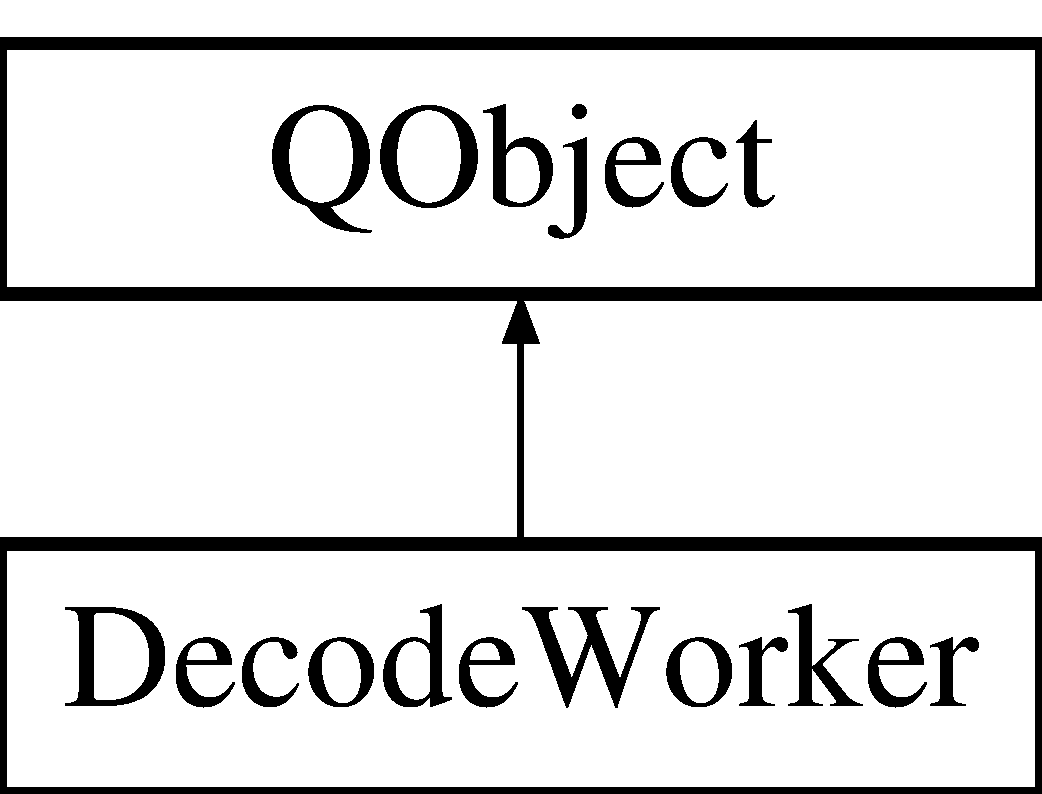
\includegraphics[height=2.000000cm]{classDecodeWorker}
\end{center}
\end{figure}
\subsection*{Public Slots}
\begin{DoxyCompactItemize}
\item 
void \hyperlink{classDecodeWorker_a12b8b121cb1745f5a88e8f8df16eee87}{decode} (int frames)
\begin{DoxyCompactList}\small\item\em \hyperlink{classDecodeWorker_a12b8b121cb1745f5a88e8f8df16eee87}{Decode\+Worker\+::decode} slot that decodes frames and converts them into a Q\+Graphics\+Pixmap\+Item. \end{DoxyCompactList}\end{DoxyCompactItemize}
\subsection*{Signals}
\begin{DoxyCompactItemize}
\item 
void {\bfseries result\+Ready} (Q\+Graphics\+Pixmap\+Item $\ast$image, int frame)\hypertarget{classDecodeWorker_a1f70e9b7ed81691577e5db962653bcc2}{}\label{classDecodeWorker_a1f70e9b7ed81691577e5db962653bcc2}

\end{DoxyCompactItemize}
\subsection*{Public Member Functions}
\begin{DoxyCompactItemize}
\item 
double {\bfseries pos\+M\+Sec} () const \hypertarget{classDecodeWorker_a59558b70a06566371f5b21b0c173cdd5}{}\label{classDecodeWorker_a59558b70a06566371f5b21b0c173cdd5}

\item 
double {\bfseries pos\+Frames} () const \hypertarget{classDecodeWorker_a2abfa502c10abf0af86a345ef459d2d2}{}\label{classDecodeWorker_a2abfa502c10abf0af86a345ef459d2d2}

\item 
void \hyperlink{classDecodeWorker_a485dae2b43c26af4832bccf8a2eaa3e4}{set\+Pos\+Frames} (double frame)
\begin{DoxyCompactList}\small\item\em \hyperlink{classDecodeWorker_a485dae2b43c26af4832bccf8a2eaa3e4}{Decode\+Worker\+::set\+Pos\+Frames} sets the Current Frame of the decoder to frame. \end{DoxyCompactList}\item 
double {\bfseries pos\+Relative} () const \hypertarget{classDecodeWorker_a1655a4700f7c4bbce116d51b43d00460}{}\label{classDecodeWorker_a1655a4700f7c4bbce116d51b43d00460}

\item 
double {\bfseries framerate} () const \hypertarget{classDecodeWorker_a08837d85e00320eb7f1b6ca665183c9e}{}\label{classDecodeWorker_a08837d85e00320eb7f1b6ca665183c9e}

\item 
double {\bfseries codec} () const \hypertarget{classDecodeWorker_aacd4b1b5e2e6535bcc89e4600666d357}{}\label{classDecodeWorker_aacd4b1b5e2e6535bcc89e4600666d357}

\item 
double {\bfseries frame\+Count} () const \hypertarget{classDecodeWorker_a859f0abdaf0e932e1b4349b496dce273}{}\label{classDecodeWorker_a859f0abdaf0e932e1b4349b496dce273}

\item 
bool \hyperlink{classDecodeWorker_a4bbc60cd77f71a0c52b06a56e4b84622}{open\+Stream} (Q\+String stream)
\begin{DoxyCompactList}\small\item\em \hyperlink{classDecodeWorker_a4bbc60cd77f71a0c52b06a56e4b84622}{Decode\+Worker\+::open\+Stream} opens stream. \end{DoxyCompactList}\item 
void \hyperlink{classDecodeWorker_a64fe44b112f634f847f0c68123680cd6}{update\+All\+Properties} ()\hypertarget{classDecodeWorker_a64fe44b112f634f847f0c68123680cd6}{}\label{classDecodeWorker_a64fe44b112f634f847f0c68123680cd6}

\begin{DoxyCompactList}\small\item\em \hyperlink{classDecodeWorker_a64fe44b112f634f847f0c68123680cd6}{Decode\+Worker\+::update\+All\+Properties} updated every property that can be accessed. \end{DoxyCompactList}\end{DoxyCompactItemize}


\subsection{Member Function Documentation}
\index{Decode\+Worker@{Decode\+Worker}!decode@{decode}}
\index{decode@{decode}!Decode\+Worker@{Decode\+Worker}}
\subsubsection[{\texorpdfstring{decode}{decode}}]{\setlength{\rightskip}{0pt plus 5cm}void Decode\+Worker\+::decode (
\begin{DoxyParamCaption}
\item[{int}]{frames}
\end{DoxyParamCaption}
)\hspace{0.3cm}{\ttfamily [slot]}}\hypertarget{classDecodeWorker_a12b8b121cb1745f5a88e8f8df16eee87}{}\label{classDecodeWorker_a12b8b121cb1745f5a88e8f8df16eee87}


\hyperlink{classDecodeWorker_a12b8b121cb1745f5a88e8f8df16eee87}{Decode\+Worker\+::decode} slot that decodes frames and converts them into a Q\+Graphics\+Pixmap\+Item. 


\begin{DoxyParams}{Parameters}
{\em frames} & \\
\hline
\end{DoxyParams}
\index{Decode\+Worker@{Decode\+Worker}!open\+Stream@{open\+Stream}}
\index{open\+Stream@{open\+Stream}!Decode\+Worker@{Decode\+Worker}}
\subsubsection[{\texorpdfstring{open\+Stream(\+Q\+String stream)}{openStream(QString stream)}}]{\setlength{\rightskip}{0pt plus 5cm}bool Decode\+Worker\+::open\+Stream (
\begin{DoxyParamCaption}
\item[{Q\+String}]{stream}
\end{DoxyParamCaption}
)}\hypertarget{classDecodeWorker_a4bbc60cd77f71a0c52b06a56e4b84622}{}\label{classDecodeWorker_a4bbc60cd77f71a0c52b06a56e4b84622}


\hyperlink{classDecodeWorker_a4bbc60cd77f71a0c52b06a56e4b84622}{Decode\+Worker\+::open\+Stream} opens stream. 


\begin{DoxyParams}{Parameters}
{\em stream} & filename of the stream \\
\hline
\end{DoxyParams}
\begin{DoxyReturn}{Returns}
true when successfull 
\end{DoxyReturn}
\index{Decode\+Worker@{Decode\+Worker}!set\+Pos\+Frames@{set\+Pos\+Frames}}
\index{set\+Pos\+Frames@{set\+Pos\+Frames}!Decode\+Worker@{Decode\+Worker}}
\subsubsection[{\texorpdfstring{set\+Pos\+Frames(double frame)}{setPosFrames(double frame)}}]{\setlength{\rightskip}{0pt plus 5cm}void Decode\+Worker\+::set\+Pos\+Frames (
\begin{DoxyParamCaption}
\item[{double}]{frame}
\end{DoxyParamCaption}
)}\hypertarget{classDecodeWorker_a485dae2b43c26af4832bccf8a2eaa3e4}{}\label{classDecodeWorker_a485dae2b43c26af4832bccf8a2eaa3e4}


\hyperlink{classDecodeWorker_a485dae2b43c26af4832bccf8a2eaa3e4}{Decode\+Worker\+::set\+Pos\+Frames} sets the Current Frame of the decoder to frame. 


\begin{DoxyParams}{Parameters}
{\em frame} & \\
\hline
\end{DoxyParams}


The documentation for this class was generated from the following files\+:\begin{DoxyCompactItemize}
\item 
decode\+\_\+worker.\+h\item 
decode\+\_\+worker.\+cpp\end{DoxyCompactItemize}

\hypertarget{classMainWindow}{}\section{Main\+Window Class Reference}
\label{classMainWindow}\index{Main\+Window@{Main\+Window}}
Inheritance diagram for Main\+Window\+:\begin{figure}[H]
\begin{center}
\leavevmode
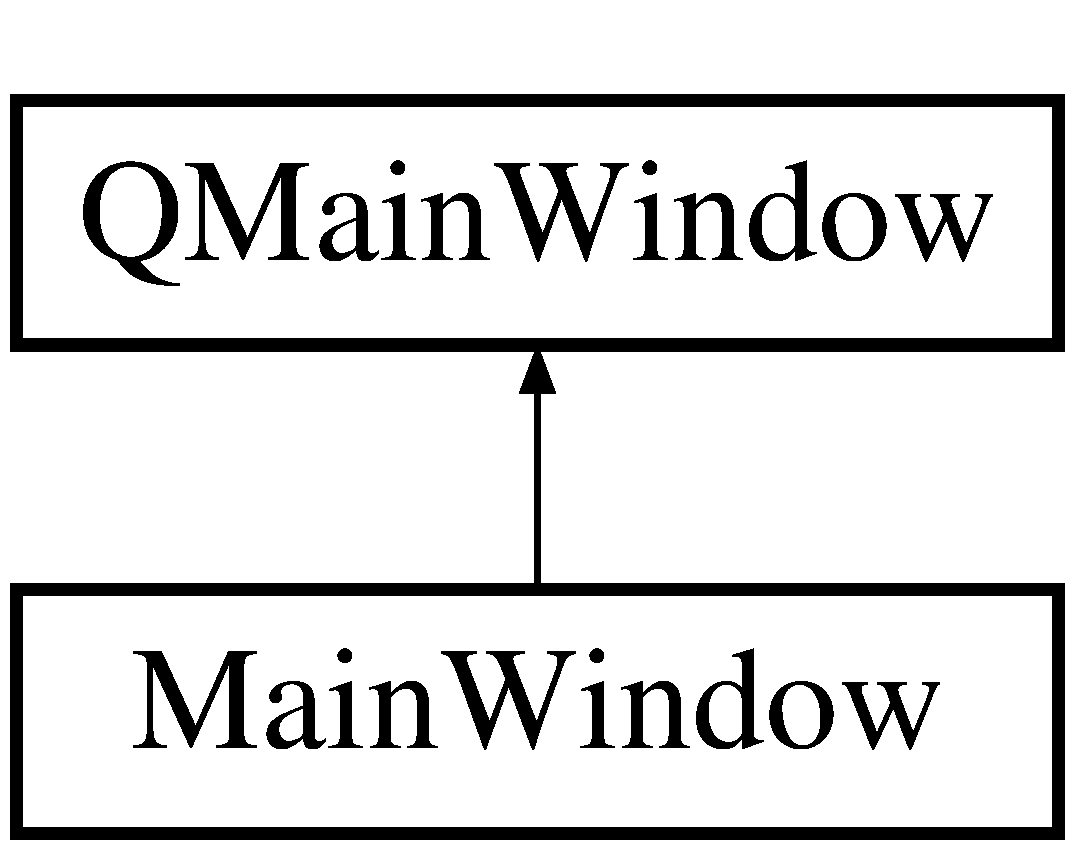
\includegraphics[height=2.000000cm]{classMainWindow}
\end{center}
\end{figure}
\subsection*{Signals}
\begin{DoxyCompactItemize}
\item 
void \hyperlink{classMainWindow_a97826b0f39a7c296aba75f34123f3c82}{freed\+Images} ()\hypertarget{classMainWindow_a97826b0f39a7c296aba75f34123f3c82}{}\label{classMainWindow_a97826b0f39a7c296aba75f34123f3c82}

\begin{DoxyCompactList}\small\item\em freed\+Images The scene no longer holds ownership of any image \end{DoxyCompactList}\end{DoxyCompactItemize}
\subsection*{Public Member Functions}
\begin{DoxyCompactItemize}
\item 
{\bfseries Main\+Window} (Q\+Widget $\ast$parent=0)\hypertarget{classMainWindow_a8b244be8b7b7db1b08de2a2acb9409db}{}\label{classMainWindow_a8b244be8b7b7db1b08de2a2acb9409db}

\end{DoxyCompactItemize}


The documentation for this class was generated from the following files\+:\begin{DoxyCompactItemize}
\item 
mainwindow.\+h\item 
mainwindow.\+cpp\end{DoxyCompactItemize}

\hypertarget{classOverlay}{}\section{Overlay Class Reference}
\label{classOverlay}\index{Overlay@{Overlay}}
Inheritance diagram for Overlay\+:\begin{figure}[H]
\begin{center}
\leavevmode
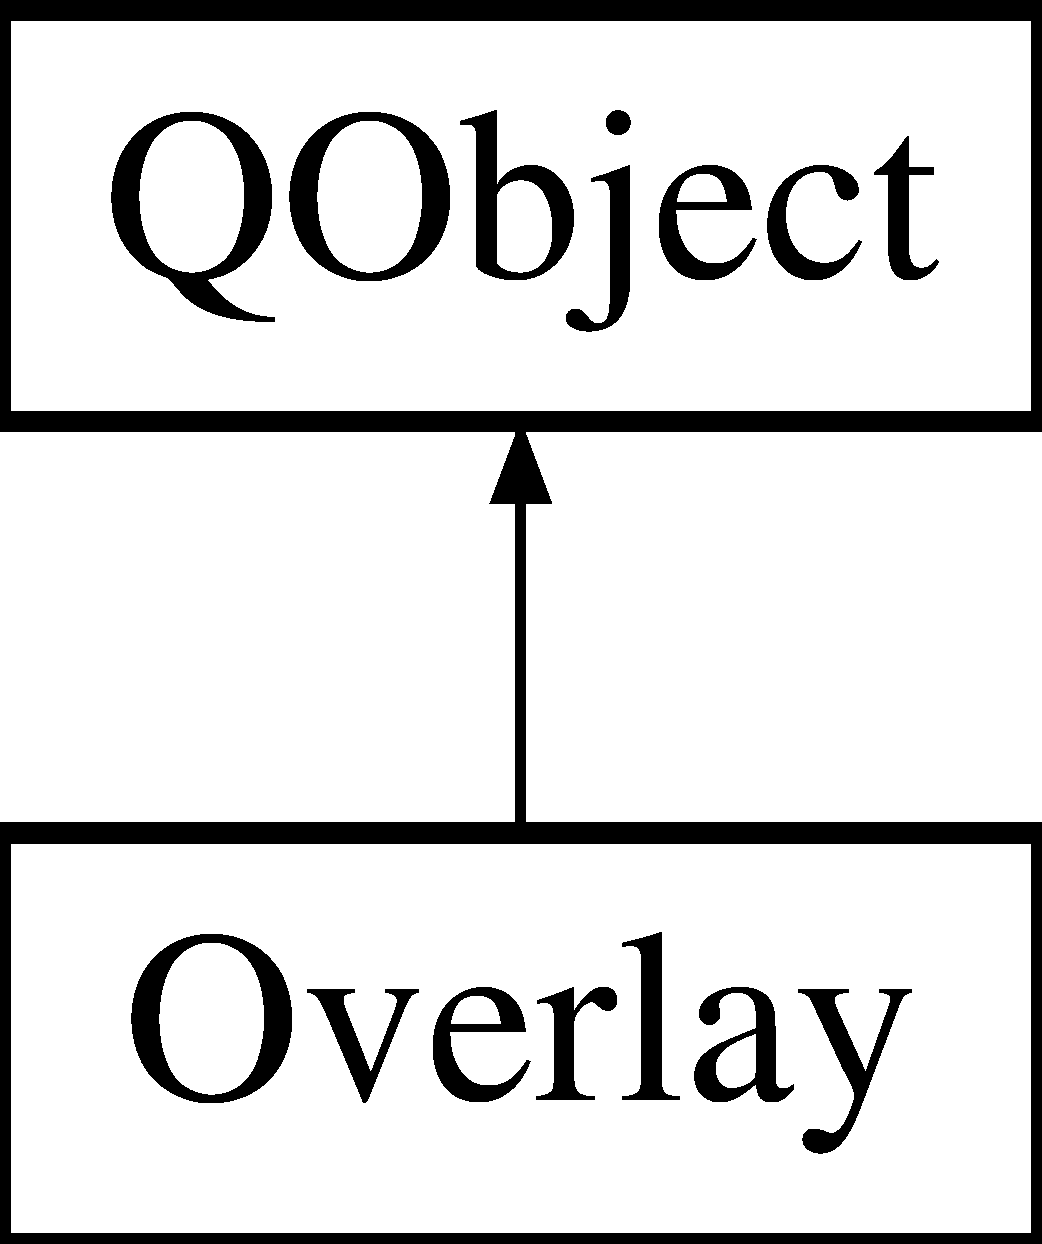
\includegraphics[height=2.000000cm]{classOverlay}
\end{center}
\end{figure}
\subsection*{Public Types}
\begin{DoxyCompactItemize}
\item 
enum \hyperlink{classOverlay_a9ef00f03a1372dc5bf0ae9b399c18193}{Parser\+Error} \{ \hyperlink{classOverlay_a9ef00f03a1372dc5bf0ae9b399c18193ae7066bd6638ef675ab94e1c083cb1bd0}{No\+Error}, 
\hyperlink{classOverlay_a9ef00f03a1372dc5bf0ae9b399c18193a1784694bdc240ab419e6178291eaa399}{Open\+File\+Error}, 
{\bfseries Parse\+Error}
 \}\begin{DoxyCompactList}\small\item\em Overlay\+::\+Parse\+Error Enum for storing euccess of parsing. \end{DoxyCompactList}
\end{DoxyCompactItemize}
\subsection*{Public Member Functions}
\begin{DoxyCompactItemize}
\item 
Q\+Pair$<$ Q\+Vector2D, qint64 $>$ \hyperlink{classOverlay_a921b608d3714021e122fde3d153f506a}{next\+Overlay} (quint32 \hyperlink{classOverlay_aba30f4cadbcfead2b1b44915617f0d32}{time\+Stamp})
\begin{DoxyCompactList}\small\item\em \hyperlink{classOverlay_a921b608d3714021e122fde3d153f506a}{Overlay\+::next\+Overlay} gets the next overlay after time\+Stamp. \end{DoxyCompactList}\item 
Q\+Pair$<$ Q\+Vector2D, qint64 $>$ \hyperlink{classOverlay_a08d7f62632a8b2e64a8bb0e9c2860cd3}{next\+Overlay} ()
\begin{DoxyCompactList}\small\item\em \hyperlink{classOverlay_a921b608d3714021e122fde3d153f506a}{Overlay\+::next\+Overlay} gets the next overlay after a time\+Stamp that is internaly stored. \end{DoxyCompactList}\item 
Q\+Pair$<$ Q\+Vector2D, qint64 $>$ \hyperlink{classOverlay_ae47a6d898295796503682a65ea31ae41}{previous\+Overlay} (quint32 \hyperlink{classOverlay_aba30f4cadbcfead2b1b44915617f0d32}{time\+Stamp})
\begin{DoxyCompactList}\small\item\em \hyperlink{classOverlay_ae47a6d898295796503682a65ea31ae41}{Overlay\+::previous\+Overlay} gets the previous overlay before time\+Stamp. \end{DoxyCompactList}\item 
Q\+Pair$<$ Q\+Vector2D, qint64 $>$ \hyperlink{classOverlay_abc4a1e11befa7b8f4cf639d7528c3e27}{previous\+Overlay} ()
\begin{DoxyCompactList}\small\item\em \hyperlink{classOverlay_ae47a6d898295796503682a65ea31ae41}{Overlay\+::previous\+Overlay} gets the previous overlay before a time\+Stamp that is internaly stored. \end{DoxyCompactList}\item 
Q\+Vector$<$ Q\+Vector2D $>$ \hyperlink{classOverlay_a64f4cbdcaab04599465bc4381c134646}{overlays\+To\+Frame} (int \hyperlink{classOverlay_a39d037dcbfcdc8f2aaa39951bcd9acfc}{frame})
\begin{DoxyCompactList}\small\item\em \hyperlink{classOverlay_a64f4cbdcaab04599465bc4381c134646}{Overlay\+::overlays\+To\+Frame}. \end{DoxyCompactList}\item 
\hyperlink{classOverlay_a9ef00f03a1372dc5bf0ae9b399c18193}{Overlay\+::\+Parser\+Error} \hyperlink{classOverlay_add3d9864ecc33df3f599e163c11fcb6d}{parse\+Overlays} (Q\+String file\+Name)
\begin{DoxyCompactList}\small\item\em \hyperlink{classOverlay_add3d9864ecc33df3f599e163c11fcb6d}{Overlay\+::parse\+Overlays} parses the content of file\+Name as overlays. Each line that has more or equal to 3 tab separated values and doesn start with \textquotesingle{}\#\textquotesingle{} is parsed. \end{DoxyCompactList}\item 
\hyperlink{classOverlay_a9ef00f03a1372dc5bf0ae9b399c18193}{Overlay\+::\+Parser\+Error} \hyperlink{classOverlay_ac7f1e54f1d27a7ad0c7991dd8afb88f4}{parse\+Frames} (Q\+String file\+Name)
\begin{DoxyCompactList}\small\item\em \hyperlink{classOverlay_ac7f1e54f1d27a7ad0c7991dd8afb88f4}{Overlay\+::parse\+Frames} parses the content of file\+Name as timestamp. Each line that has more or equal to 1 tab separated values and doesn start with \textquotesingle{}\#\textquotesingle{} is parsed. \end{DoxyCompactList}\item 
qint64 \hyperlink{classOverlay_aba30f4cadbcfead2b1b44915617f0d32}{time\+Stamp} (int \hyperlink{classOverlay_a39d037dcbfcdc8f2aaa39951bcd9acfc}{frame})
\begin{DoxyCompactList}\small\item\em \hyperlink{classOverlay_aba30f4cadbcfead2b1b44915617f0d32}{Overlay\+::time\+Stamp} returns the timestamp to frame in constant time. \end{DoxyCompactList}\item 
int \hyperlink{classOverlay_a39d037dcbfcdc8f2aaa39951bcd9acfc}{frame} (quint32 timestamp)
\begin{DoxyCompactList}\small\item\em \hyperlink{classOverlay_a39d037dcbfcdc8f2aaa39951bcd9acfc}{Overlay\+::frame} returns the next lower framenumber that comes before timestamp This is done in logarithmic time. \end{DoxyCompactList}\end{DoxyCompactItemize}


\subsection{Member Enumeration Documentation}
\index{Overlay@{Overlay}!Parser\+Error@{Parser\+Error}}
\index{Parser\+Error@{Parser\+Error}!Overlay@{Overlay}}
\subsubsection[{\texorpdfstring{Parser\+Error}{ParserError}}]{\setlength{\rightskip}{0pt plus 5cm}enum {\bf Overlay\+::\+Parser\+Error}}\hypertarget{classOverlay_a9ef00f03a1372dc5bf0ae9b399c18193}{}\label{classOverlay_a9ef00f03a1372dc5bf0ae9b399c18193}


Overlay\+::\+Parse\+Error Enum for storing euccess of parsing. 

\begin{Desc}
\item[Enumerator]\par
\begin{description}
\index{No\+Error@{No\+Error}!Overlay@{Overlay}}\index{Overlay@{Overlay}!No\+Error@{No\+Error}}\item[{\em 
No\+Error\hypertarget{classOverlay_a9ef00f03a1372dc5bf0ae9b399c18193ae7066bd6638ef675ab94e1c083cb1bd0}{}\label{classOverlay_a9ef00f03a1372dc5bf0ae9b399c18193ae7066bd6638ef675ab94e1c083cb1bd0}
}]Parsing was successfull. \index{Open\+File\+Error@{Open\+File\+Error}!Overlay@{Overlay}}\index{Overlay@{Overlay}!Open\+File\+Error@{Open\+File\+Error}}\item[{\em 
Open\+File\+Error\hypertarget{classOverlay_a9ef00f03a1372dc5bf0ae9b399c18193a1784694bdc240ab419e6178291eaa399}{}\label{classOverlay_a9ef00f03a1372dc5bf0ae9b399c18193a1784694bdc240ab419e6178291eaa399}
}]Could not open File to parse. \end{description}
\end{Desc}


\subsection{Member Function Documentation}
\index{Overlay@{Overlay}!frame@{frame}}
\index{frame@{frame}!Overlay@{Overlay}}
\subsubsection[{\texorpdfstring{frame(quint32 timestamp)}{frame(quint32 timestamp)}}]{\setlength{\rightskip}{0pt plus 5cm}int Overlay\+::frame (
\begin{DoxyParamCaption}
\item[{quint32}]{timestamp}
\end{DoxyParamCaption}
)}\hypertarget{classOverlay_a39d037dcbfcdc8f2aaa39951bcd9acfc}{}\label{classOverlay_a39d037dcbfcdc8f2aaa39951bcd9acfc}


\hyperlink{classOverlay_a39d037dcbfcdc8f2aaa39951bcd9acfc}{Overlay\+::frame} returns the next lower framenumber that comes before timestamp This is done in logarithmic time. 


\begin{DoxyParams}{Parameters}
{\em timestamp} & used as a threshold \\
\hline
\end{DoxyParams}
\begin{DoxyReturn}{Returns}
framenumber, always between 0 and the amount of parsed Frames 
\end{DoxyReturn}
\index{Overlay@{Overlay}!next\+Overlay@{next\+Overlay}}
\index{next\+Overlay@{next\+Overlay}!Overlay@{Overlay}}
\subsubsection[{\texorpdfstring{next\+Overlay(quint32 time\+Stamp)}{nextOverlay(quint32 timeStamp)}}]{\setlength{\rightskip}{0pt plus 5cm}Q\+Pair$<$ Q\+Vector2D, qint64 $>$ Overlay\+::next\+Overlay (
\begin{DoxyParamCaption}
\item[{quint32}]{time\+Stamp}
\end{DoxyParamCaption}
)}\hypertarget{classOverlay_a921b608d3714021e122fde3d153f506a}{}\label{classOverlay_a921b608d3714021e122fde3d153f506a}


\hyperlink{classOverlay_a921b608d3714021e122fde3d153f506a}{Overlay\+::next\+Overlay} gets the next overlay after time\+Stamp. 


\begin{DoxyParams}{Parameters}
{\em time\+Stamp} & \\
\hline
\end{DoxyParams}
\begin{DoxyReturn}{Returns}
position and timestamp of the next overlay after time\+Stamp If there is no next \hyperlink{classOverlay}{Overlay} after time\+Stamp the function returns -\/1 as time\+Stamp 
\end{DoxyReturn}
\index{Overlay@{Overlay}!next\+Overlay@{next\+Overlay}}
\index{next\+Overlay@{next\+Overlay}!Overlay@{Overlay}}
\subsubsection[{\texorpdfstring{next\+Overlay()}{nextOverlay()}}]{\setlength{\rightskip}{0pt plus 5cm}Q\+Pair$<$ Q\+Vector2D, qint64 $>$ Overlay\+::next\+Overlay (
\begin{DoxyParamCaption}
{}
\end{DoxyParamCaption}
)}\hypertarget{classOverlay_a08d7f62632a8b2e64a8bb0e9c2860cd3}{}\label{classOverlay_a08d7f62632a8b2e64a8bb0e9c2860cd3}


\hyperlink{classOverlay_a921b608d3714021e122fde3d153f506a}{Overlay\+::next\+Overlay} gets the next overlay after a time\+Stamp that is internaly stored. 

\begin{DoxyReturn}{Returns}
position and timestamp of the next overlay after time\+Stamp If there is no next \hyperlink{classOverlay}{Overlay} after an internal stored timestamp the function returns -\/1 as time\+Stamp 
\end{DoxyReturn}
\index{Overlay@{Overlay}!overlays\+To\+Frame@{overlays\+To\+Frame}}
\index{overlays\+To\+Frame@{overlays\+To\+Frame}!Overlay@{Overlay}}
\subsubsection[{\texorpdfstring{overlays\+To\+Frame(int frame)}{overlaysToFrame(int frame)}}]{\setlength{\rightskip}{0pt plus 5cm}Q\+Vector$<$ Q\+Vector2D $>$ Overlay\+::overlays\+To\+Frame (
\begin{DoxyParamCaption}
\item[{int}]{frame}
\end{DoxyParamCaption}
)}\hypertarget{classOverlay_a64f4cbdcaab04599465bc4381c134646}{}\label{classOverlay_a64f4cbdcaab04599465bc4381c134646}


\hyperlink{classOverlay_a64f4cbdcaab04599465bc4381c134646}{Overlay\+::overlays\+To\+Frame}. 


\begin{DoxyParams}{Parameters}
{\em frame} & framenumber \\
\hline
\end{DoxyParams}
\begin{DoxyReturn}{Returns}
All overlays that have a timestamp between the timestamp of frame and the next frame as a Q\+Vector 
\end{DoxyReturn}
\index{Overlay@{Overlay}!parse\+Frames@{parse\+Frames}}
\index{parse\+Frames@{parse\+Frames}!Overlay@{Overlay}}
\subsubsection[{\texorpdfstring{parse\+Frames(\+Q\+String file\+Name)}{parseFrames(QString fileName)}}]{\setlength{\rightskip}{0pt plus 5cm}{\bf Overlay\+::\+Parser\+Error} Overlay\+::parse\+Frames (
\begin{DoxyParamCaption}
\item[{Q\+String}]{file\+Name}
\end{DoxyParamCaption}
)}\hypertarget{classOverlay_ac7f1e54f1d27a7ad0c7991dd8afb88f4}{}\label{classOverlay_ac7f1e54f1d27a7ad0c7991dd8afb88f4}


\hyperlink{classOverlay_ac7f1e54f1d27a7ad0c7991dd8afb88f4}{Overlay\+::parse\+Frames} parses the content of file\+Name as timestamp. Each line that has more or equal to 1 tab separated values and doesn start with \textquotesingle{}\#\textquotesingle{} is parsed. 


\begin{DoxyParams}{Parameters}
{\em file\+Name} & Path to the file that is to be parsed \\
\hline
\end{DoxyParams}
\begin{DoxyReturn}{Returns}
Parser\+Error Open\+File\+Error when it isn\textquotesingle{}t possible to open the file Parse\+Error when the parser failed to parse any line or a line contained invalid characters Noerror when the parser could parse the file successfuly 
\end{DoxyReturn}
\index{Overlay@{Overlay}!parse\+Overlays@{parse\+Overlays}}
\index{parse\+Overlays@{parse\+Overlays}!Overlay@{Overlay}}
\subsubsection[{\texorpdfstring{parse\+Overlays(\+Q\+String file\+Name)}{parseOverlays(QString fileName)}}]{\setlength{\rightskip}{0pt plus 5cm}{\bf Overlay\+::\+Parser\+Error} Overlay\+::parse\+Overlays (
\begin{DoxyParamCaption}
\item[{Q\+String}]{file\+Name}
\end{DoxyParamCaption}
)}\hypertarget{classOverlay_add3d9864ecc33df3f599e163c11fcb6d}{}\label{classOverlay_add3d9864ecc33df3f599e163c11fcb6d}


\hyperlink{classOverlay_add3d9864ecc33df3f599e163c11fcb6d}{Overlay\+::parse\+Overlays} parses the content of file\+Name as overlays. Each line that has more or equal to 3 tab separated values and doesn start with \textquotesingle{}\#\textquotesingle{} is parsed. 


\begin{DoxyParams}{Parameters}
{\em file\+Name} & Path to the file that is to be parsed \\
\hline
\end{DoxyParams}
\begin{DoxyReturn}{Returns}
Parser\+Error Open\+File\+Error when it isn\textquotesingle{}t possible to open the file Parse\+Error when the parser failed to parse any line or a line contained invalid characters Noerror when the parser could parse the file successfuly 
\end{DoxyReturn}
\index{Overlay@{Overlay}!previous\+Overlay@{previous\+Overlay}}
\index{previous\+Overlay@{previous\+Overlay}!Overlay@{Overlay}}
\subsubsection[{\texorpdfstring{previous\+Overlay(quint32 time\+Stamp)}{previousOverlay(quint32 timeStamp)}}]{\setlength{\rightskip}{0pt plus 5cm}Q\+Pair$<$ Q\+Vector2D, qint64 $>$ Overlay\+::previous\+Overlay (
\begin{DoxyParamCaption}
\item[{quint32}]{time\+Stamp}
\end{DoxyParamCaption}
)}\hypertarget{classOverlay_ae47a6d898295796503682a65ea31ae41}{}\label{classOverlay_ae47a6d898295796503682a65ea31ae41}


\hyperlink{classOverlay_ae47a6d898295796503682a65ea31ae41}{Overlay\+::previous\+Overlay} gets the previous overlay before time\+Stamp. 


\begin{DoxyParams}{Parameters}
{\em time\+Stamp} & \\
\hline
\end{DoxyParams}
\begin{DoxyReturn}{Returns}
position and timestamp of the previous overlay before time\+Stamp If there is no previous \hyperlink{classOverlay}{Overlay} before time\+Stamp the function returns -\/1 as time\+Stamp 
\end{DoxyReturn}
\index{Overlay@{Overlay}!previous\+Overlay@{previous\+Overlay}}
\index{previous\+Overlay@{previous\+Overlay}!Overlay@{Overlay}}
\subsubsection[{\texorpdfstring{previous\+Overlay()}{previousOverlay()}}]{\setlength{\rightskip}{0pt plus 5cm}Q\+Pair$<$ Q\+Vector2D, qint64 $>$ Overlay\+::previous\+Overlay (
\begin{DoxyParamCaption}
{}
\end{DoxyParamCaption}
)}\hypertarget{classOverlay_abc4a1e11befa7b8f4cf639d7528c3e27}{}\label{classOverlay_abc4a1e11befa7b8f4cf639d7528c3e27}


\hyperlink{classOverlay_ae47a6d898295796503682a65ea31ae41}{Overlay\+::previous\+Overlay} gets the previous overlay before a time\+Stamp that is internaly stored. 

\begin{DoxyReturn}{Returns}
position and timestamp of the previous overlay before time\+Stamp If there is no previous \hyperlink{classOverlay}{Overlay} before an internal stored timestamp the function returns -\/1 as time\+Stamp 
\end{DoxyReturn}
\index{Overlay@{Overlay}!time\+Stamp@{time\+Stamp}}
\index{time\+Stamp@{time\+Stamp}!Overlay@{Overlay}}
\subsubsection[{\texorpdfstring{time\+Stamp(int frame)}{timeStamp(int frame)}}]{\setlength{\rightskip}{0pt plus 5cm}qint64 Overlay\+::time\+Stamp (
\begin{DoxyParamCaption}
\item[{int}]{frame}
\end{DoxyParamCaption}
)}\hypertarget{classOverlay_aba30f4cadbcfead2b1b44915617f0d32}{}\label{classOverlay_aba30f4cadbcfead2b1b44915617f0d32}


\hyperlink{classOverlay_aba30f4cadbcfead2b1b44915617f0d32}{Overlay\+::time\+Stamp} returns the timestamp to frame in constant time. 


\begin{DoxyParams}{Parameters}
{\em frame} & \\
\hline
\end{DoxyParams}
\begin{DoxyReturn}{Returns}
timestamp of frame with framenumber frame, -\/1 if frame is not available 
\end{DoxyReturn}


The documentation for this class was generated from the following files\+:\begin{DoxyCompactItemize}
\item 
overlay.\+h\item 
overlay.\+cpp\end{DoxyCompactItemize}

\hypertarget{classVideoHandler}{}\section{Video\+Handler Class Reference}
\label{classVideoHandler}\index{Video\+Handler@{Video\+Handler}}


The \hyperlink{classVideoHandler}{Video\+Handler} class handles when each frame and overlay gets displayed on screen synchronized, handles the video buffer, requests frames as needed, allows controll of the playback.  




{\ttfamily \#include $<$video\+\_\+handler.\+h$>$}

Inheritance diagram for Video\+Handler\+:\begin{figure}[H]
\begin{center}
\leavevmode
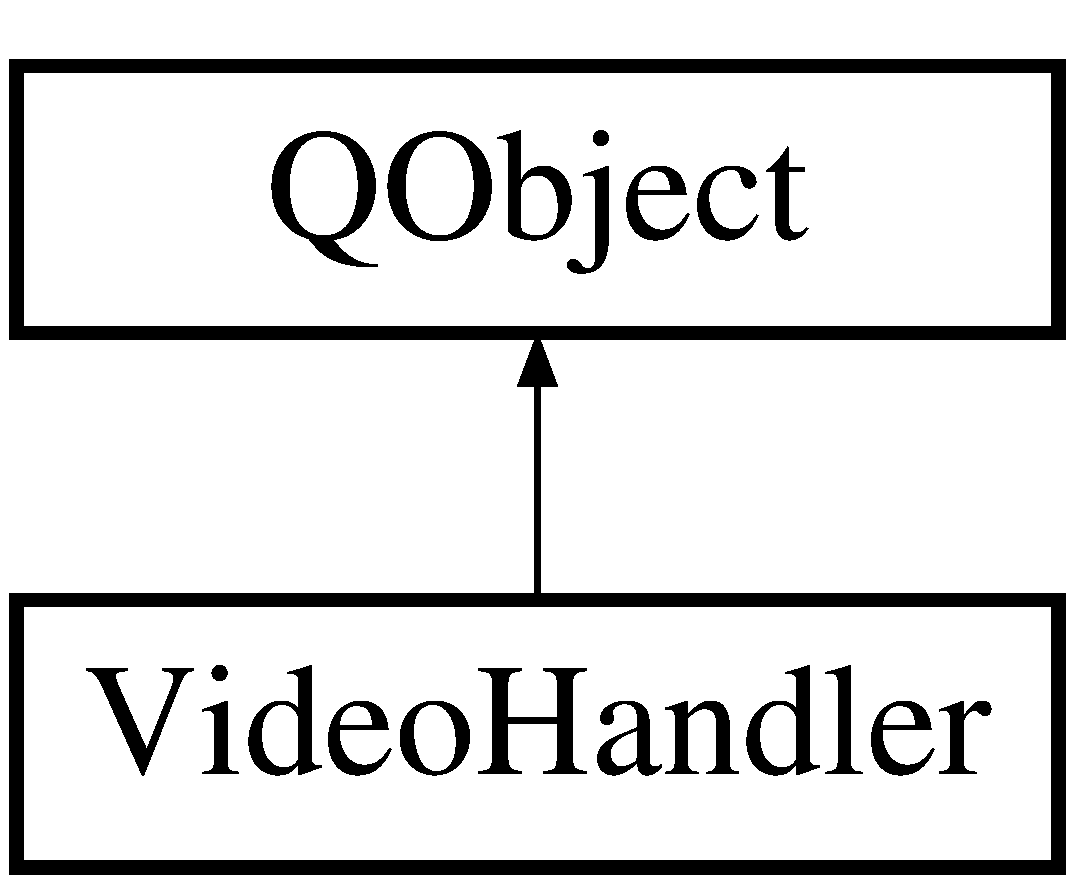
\includegraphics[height=2.000000cm]{classVideoHandler}
\end{center}
\end{figure}
\subsection*{Public Types}
\begin{DoxyCompactItemize}
\item 
enum {\bfseries Play\+State} \{ {\bfseries pause}, 
{\bfseries play\+Video}, 
{\bfseries play\+Overlays}
 \}\hypertarget{classVideoHandler_a2b1835a79f75fd56eadac477d3652b91}{}\label{classVideoHandler_a2b1835a79f75fd56eadac477d3652b91}

\end{DoxyCompactItemize}
\subsection*{Public Slots}
\begin{DoxyCompactItemize}
\item 
void \hyperlink{classVideoHandler_a453238d48cf43f92da176366e0aace6f}{play} ()\hypertarget{classVideoHandler_a453238d48cf43f92da176366e0aace6f}{}\label{classVideoHandler_a453238d48cf43f92da176366e0aace6f}

\begin{DoxyCompactList}\small\item\em \hyperlink{classVideoHandler_a453238d48cf43f92da176366e0aace6f}{Video\+Handler\+::play} starts video playback with normal speed If the video is already playing it pauses the playback. \end{DoxyCompactList}\item 
void \hyperlink{classVideoHandler_a7e80d78cb9c2514a2b19c285ddcdd42d}{play\+Overlay} ()\hypertarget{classVideoHandler_a7e80d78cb9c2514a2b19c285ddcdd42d}{}\label{classVideoHandler_a7e80d78cb9c2514a2b19c285ddcdd42d}

\begin{DoxyCompactList}\small\item\em \hyperlink{classVideoHandler_a7e80d78cb9c2514a2b19c285ddcdd42d}{Video\+Handler\+::play\+Overlay} starts the playback of the overlays with the speed of the normal video. If the overlays are already playing it will pause the playback. \end{DoxyCompactList}\item 
void \hyperlink{classVideoHandler_af9c6426d96227ffd38c0b7db6aaf037d}{timeout} ()\hypertarget{classVideoHandler_af9c6426d96227ffd38c0b7db6aaf037d}{}\label{classVideoHandler_af9c6426d96227ffd38c0b7db6aaf037d}

\begin{DoxyCompactList}\small\item\em \hyperlink{classVideoHandler_af9c6426d96227ffd38c0b7db6aaf037d}{Video\+Handler\+::timeout} slot that gets called if a new frame or overlay needs to be displayed. Reduces the buffer size to 50 Images if the buffer is bigger than 100 Images. \end{DoxyCompactList}\item 
void \hyperlink{classVideoHandler_aaa4f41896e565606552d960951145ca5}{open} ()\hypertarget{classVideoHandler_aaa4f41896e565606552d960951145ca5}{}\label{classVideoHandler_aaa4f41896e565606552d960951145ca5}

\begin{DoxyCompactList}\small\item\em \hyperlink{classVideoHandler_aaa4f41896e565606552d960951145ca5}{Video\+Handler\+::open} opens a new video file and deletes all previous buffered images. \end{DoxyCompactList}\item 
void \hyperlink{classVideoHandler_a0ea54798e44864231a65bc1e9c3b502e}{open\+Overlay} ()\hypertarget{classVideoHandler_a0ea54798e44864231a65bc1e9c3b502e}{}\label{classVideoHandler_a0ea54798e44864231a65bc1e9c3b502e}

\begin{DoxyCompactList}\small\item\em \hyperlink{classVideoHandler_a0ea54798e44864231a65bc1e9c3b502e}{Video\+Handler\+::open\+Overlay} opens a csv file and parses it. \end{DoxyCompactList}\item 
void \hyperlink{classVideoHandler_a31fd29045a8a75b4daad184dd1ddb49e}{open\+Timestamp} ()\hypertarget{classVideoHandler_a31fd29045a8a75b4daad184dd1ddb49e}{}\label{classVideoHandler_a31fd29045a8a75b4daad184dd1ddb49e}

\begin{DoxyCompactList}\small\item\em \hyperlink{classVideoHandler_a31fd29045a8a75b4daad184dd1ddb49e}{Video\+Handler\+::open\+Timestamp} Opens timestamp file and parses the file. \end{DoxyCompactList}\item 
void \hyperlink{classVideoHandler_a19f870ae02d495c88c5ed52eba0abc9e}{image\+Freed} ()\hypertarget{classVideoHandler_a19f870ae02d495c88c5ed52eba0abc9e}{}\label{classVideoHandler_a19f870ae02d495c88c5ed52eba0abc9e}

\begin{DoxyCompactList}\small\item\em \hyperlink{classVideoHandler_a19f870ae02d495c88c5ed52eba0abc9e}{Video\+Handler\+::image\+Freed} slots that gets calles when \+\_\+current\+Image and \+\_\+previous\+Image are removed from the scene. And it deletes them. \end{DoxyCompactList}\item 
void \hyperlink{classVideoHandler_ac3aa37f13e2901e830c0070bbb8aad27}{next\+Image} ()\hypertarget{classVideoHandler_ac3aa37f13e2901e830c0070bbb8aad27}{}\label{classVideoHandler_ac3aa37f13e2901e830c0070bbb8aad27}

\begin{DoxyCompactList}\small\item\em \hyperlink{classVideoHandler_ac3aa37f13e2901e830c0070bbb8aad27}{Video\+Handler\+::next\+Image} slot that sends the next image and updates the overlay. \end{DoxyCompactList}\item 
void \hyperlink{classVideoHandler_a9740f6544f2695785ee84959719da200}{next\+Overlay} ()\hypertarget{classVideoHandler_a9740f6544f2695785ee84959719da200}{}\label{classVideoHandler_a9740f6544f2695785ee84959719da200}

\begin{DoxyCompactList}\small\item\em \hyperlink{classVideoHandler_a9740f6544f2695785ee84959719da200}{Video\+Handler\+::next\+Overlay} slot that sends the next \hyperlink{classOverlay}{Overlay} and updates the Image if needed. \end{DoxyCompactList}\item 
void \hyperlink{classVideoHandler_a05c7976f85369df034128b99e13515cc}{previous\+Image} ()\hypertarget{classVideoHandler_a05c7976f85369df034128b99e13515cc}{}\label{classVideoHandler_a05c7976f85369df034128b99e13515cc}

\begin{DoxyCompactList}\small\item\em \hyperlink{classVideoHandler_a05c7976f85369df034128b99e13515cc}{Video\+Handler\+::previous\+Image} slot that sends the previous Image and updates the overlay. \end{DoxyCompactList}\item 
void \hyperlink{classVideoHandler_aa438c0abfdb8ddb54d06bf7ce68dc7bc}{previous\+Overlay} ()\hypertarget{classVideoHandler_aa438c0abfdb8ddb54d06bf7ce68dc7bc}{}\label{classVideoHandler_aa438c0abfdb8ddb54d06bf7ce68dc7bc}

\begin{DoxyCompactList}\small\item\em \hyperlink{classVideoHandler_aa438c0abfdb8ddb54d06bf7ce68dc7bc}{Video\+Handler\+::previous\+Overlay} slot that sends the previous \hyperlink{classOverlay}{Overlay} and updates the Image if needed. \end{DoxyCompactList}\end{DoxyCompactItemize}
\subsection*{Signals}
\begin{DoxyCompactItemize}
\item 
void \hyperlink{classVideoHandler_abab55d876a0733246bb93b03d9bb4e6f}{update\+Slider} (int total\+Frames)
\begin{DoxyCompactList}\small\item\em update\+Slider emitted when the slider needs to be updated \end{DoxyCompactList}\item 
void \hyperlink{classVideoHandler_ad27bed625ae493aaaeae4e141062868f}{image\+Refresh} (Q\+Graphics\+Pixmap\+Item $\ast$image)
\begin{DoxyCompactList}\small\item\em image\+Refresh emitted when the image needs to be updated \end{DoxyCompactList}\item 
void \hyperlink{classVideoHandler_afc0683e30a8dee583596e2beac972133}{overlay\+Refresh} (Q\+Point pos)
\begin{DoxyCompactList}\small\item\em overlay\+Refresh emitted when the overlay needs to be adjusted \end{DoxyCompactList}\item 
void \hyperlink{classVideoHandler_ab7b0fb78bcfb33c5b7b33716a3f3e640}{decode} (int images)
\begin{DoxyCompactList}\small\item\em decode order new frame(s) to be decoded and converted \end{DoxyCompactList}\item 
void \hyperlink{classVideoHandler_a2840450055e030beb1239a0fbe638831}{free\+Image} ()\hypertarget{classVideoHandler_a2840450055e030beb1239a0fbe638831}{}\label{classVideoHandler_a2840450055e030beb1239a0fbe638831}

\begin{DoxyCompactList}\small\item\em free\+Image request ownership of images that are displayed \end{DoxyCompactList}\end{DoxyCompactItemize}
\subsection*{Public Member Functions}
\begin{DoxyCompactItemize}
\item 
\hyperlink{classVideoHandler_ac25de5d277b6a3d8bf09df2f33df281d}{Video\+Handler} ()\hypertarget{classVideoHandler_ac25de5d277b6a3d8bf09df2f33df281d}{}\label{classVideoHandler_ac25de5d277b6a3d8bf09df2f33df281d}

\begin{DoxyCompactList}\small\item\em \hyperlink{classVideoHandler_ac25de5d277b6a3d8bf09df2f33df281d}{Video\+Handler\+::\+Video\+Handler}. \end{DoxyCompactList}\item 
double \hyperlink{classVideoHandler_acbe73f36a1f9c8e63486f40a3378bdbc}{pos\+M\+Sec} () const 
\begin{DoxyCompactList}\small\item\em \hyperlink{classVideoHandler_acbe73f36a1f9c8e63486f40a3378bdbc}{Video\+Handler\+::pos\+M\+Sec}. \end{DoxyCompactList}\item 
double \hyperlink{classVideoHandler_a8bef55832d29ab40eb707f0b931e4658}{pos\+Frames} () const 
\begin{DoxyCompactList}\small\item\em \hyperlink{classVideoHandler_a8bef55832d29ab40eb707f0b931e4658}{Video\+Handler\+::pos\+Frames}. \end{DoxyCompactList}\item 
void \hyperlink{classVideoHandler_a89ca1772249f84f62f8854670ed71024}{set\+Pos\+Frames} (double frame, bool update\+Current\+Frame=true)
\begin{DoxyCompactList}\small\item\em \hyperlink{classVideoHandler_a89ca1772249f84f62f8854670ed71024}{Video\+Handler\+::set\+Pos\+Frames}. \end{DoxyCompactList}\item 
double \hyperlink{classVideoHandler_af025d2ccbde21a6b4b7b47cda9336091}{pos\+Relative} () const 
\begin{DoxyCompactList}\small\item\em \hyperlink{classVideoHandler_af025d2ccbde21a6b4b7b47cda9336091}{Video\+Handler\+::pos\+Relative}. \end{DoxyCompactList}\item 
double \hyperlink{classVideoHandler_a195088916a016f037c73dfcea55f1a46}{framerate} () const 
\begin{DoxyCompactList}\small\item\em \hyperlink{classVideoHandler_a195088916a016f037c73dfcea55f1a46}{Video\+Handler\+::framerate}. \end{DoxyCompactList}\item 
double \hyperlink{classVideoHandler_a16bec3757877062d4c0b19de1b78f6a5}{codec} () const 
\begin{DoxyCompactList}\small\item\em \hyperlink{classVideoHandler_a16bec3757877062d4c0b19de1b78f6a5}{Video\+Handler\+::codec}. \end{DoxyCompactList}\item 
double \hyperlink{classVideoHandler_a38df67408da0a1a51b4752355683ab08}{frame\+Count} () const 
\begin{DoxyCompactList}\small\item\em \hyperlink{classVideoHandler_a38df67408da0a1a51b4752355683ab08}{Video\+Handler\+::frame\+Count}. \end{DoxyCompactList}\item 
Play\+State \hyperlink{classVideoHandler_a24b5a2bbc255cd93dcfe9d9223bd04bb}{play\+State} () const 
\begin{DoxyCompactList}\small\item\em \hyperlink{classVideoHandler_a24b5a2bbc255cd93dcfe9d9223bd04bb}{Video\+Handler\+::play\+State} returns the current play\+State of the video. \end{DoxyCompactList}\end{DoxyCompactItemize}


\subsection{Detailed Description}
The \hyperlink{classVideoHandler}{Video\+Handler} class handles when each frame and overlay gets displayed on screen synchronized, handles the video buffer, requests frames as needed, allows controll of the playback. 

\subsection{Member Function Documentation}
\index{Video\+Handler@{Video\+Handler}!codec@{codec}}
\index{codec@{codec}!Video\+Handler@{Video\+Handler}}
\subsubsection[{\texorpdfstring{codec() const }{codec() const }}]{\setlength{\rightskip}{0pt plus 5cm}double Video\+Handler\+::codec (
\begin{DoxyParamCaption}
{}
\end{DoxyParamCaption}
) const}\hypertarget{classVideoHandler_a16bec3757877062d4c0b19de1b78f6a5}{}\label{classVideoHandler_a16bec3757877062d4c0b19de1b78f6a5}


\hyperlink{classVideoHandler_a16bec3757877062d4c0b19de1b78f6a5}{Video\+Handler\+::codec}. 

\begin{DoxyReturn}{Returns}
Codec of the video that is currently decoded 
\end{DoxyReturn}
\index{Video\+Handler@{Video\+Handler}!decode@{decode}}
\index{decode@{decode}!Video\+Handler@{Video\+Handler}}
\subsubsection[{\texorpdfstring{decode}{decode}}]{\setlength{\rightskip}{0pt plus 5cm}void Video\+Handler\+::decode (
\begin{DoxyParamCaption}
\item[{int}]{images}
\end{DoxyParamCaption}
)\hspace{0.3cm}{\ttfamily [signal]}}\hypertarget{classVideoHandler_ab7b0fb78bcfb33c5b7b33716a3f3e640}{}\label{classVideoHandler_ab7b0fb78bcfb33c5b7b33716a3f3e640}


decode order new frame(s) to be decoded and converted 


\begin{DoxyParams}{Parameters}
{\em images} & count of frames to be decoded \\
\hline
\end{DoxyParams}
\index{Video\+Handler@{Video\+Handler}!frame\+Count@{frame\+Count}}
\index{frame\+Count@{frame\+Count}!Video\+Handler@{Video\+Handler}}
\subsubsection[{\texorpdfstring{frame\+Count() const }{frameCount() const }}]{\setlength{\rightskip}{0pt plus 5cm}double Video\+Handler\+::frame\+Count (
\begin{DoxyParamCaption}
{}
\end{DoxyParamCaption}
) const}\hypertarget{classVideoHandler_a38df67408da0a1a51b4752355683ab08}{}\label{classVideoHandler_a38df67408da0a1a51b4752355683ab08}


\hyperlink{classVideoHandler_a38df67408da0a1a51b4752355683ab08}{Video\+Handler\+::frame\+Count}. 

\begin{DoxyReturn}{Returns}
The total amount of frames in the current playback 
\end{DoxyReturn}
\index{Video\+Handler@{Video\+Handler}!framerate@{framerate}}
\index{framerate@{framerate}!Video\+Handler@{Video\+Handler}}
\subsubsection[{\texorpdfstring{framerate() const }{framerate() const }}]{\setlength{\rightskip}{0pt plus 5cm}double Video\+Handler\+::framerate (
\begin{DoxyParamCaption}
{}
\end{DoxyParamCaption}
) const}\hypertarget{classVideoHandler_a195088916a016f037c73dfcea55f1a46}{}\label{classVideoHandler_a195088916a016f037c73dfcea55f1a46}


\hyperlink{classVideoHandler_a195088916a016f037c73dfcea55f1a46}{Video\+Handler\+::framerate}. 

\begin{DoxyReturn}{Returns}
Framerate of the video that is currently decoded 
\end{DoxyReturn}
\index{Video\+Handler@{Video\+Handler}!image\+Refresh@{image\+Refresh}}
\index{image\+Refresh@{image\+Refresh}!Video\+Handler@{Video\+Handler}}
\subsubsection[{\texorpdfstring{image\+Refresh}{imageRefresh}}]{\setlength{\rightskip}{0pt plus 5cm}void Video\+Handler\+::image\+Refresh (
\begin{DoxyParamCaption}
\item[{Q\+Graphics\+Pixmap\+Item $\ast$}]{image}
\end{DoxyParamCaption}
)\hspace{0.3cm}{\ttfamily [signal]}}\hypertarget{classVideoHandler_ad27bed625ae493aaaeae4e141062868f}{}\label{classVideoHandler_ad27bed625ae493aaaeae4e141062868f}


image\+Refresh emitted when the image needs to be updated 


\begin{DoxyParams}{Parameters}
{\em image} & \\
\hline
\end{DoxyParams}
\index{Video\+Handler@{Video\+Handler}!overlay\+Refresh@{overlay\+Refresh}}
\index{overlay\+Refresh@{overlay\+Refresh}!Video\+Handler@{Video\+Handler}}
\subsubsection[{\texorpdfstring{overlay\+Refresh}{overlayRefresh}}]{\setlength{\rightskip}{0pt plus 5cm}void Video\+Handler\+::overlay\+Refresh (
\begin{DoxyParamCaption}
\item[{Q\+Point}]{pos}
\end{DoxyParamCaption}
)\hspace{0.3cm}{\ttfamily [signal]}}\hypertarget{classVideoHandler_afc0683e30a8dee583596e2beac972133}{}\label{classVideoHandler_afc0683e30a8dee583596e2beac972133}


overlay\+Refresh emitted when the overlay needs to be adjusted 


\begin{DoxyParams}{Parameters}
{\em pos} & \\
\hline
\end{DoxyParams}
\index{Video\+Handler@{Video\+Handler}!play\+State@{play\+State}}
\index{play\+State@{play\+State}!Video\+Handler@{Video\+Handler}}
\subsubsection[{\texorpdfstring{play\+State() const }{playState() const }}]{\setlength{\rightskip}{0pt plus 5cm}Video\+Handler\+::\+Play\+State Video\+Handler\+::play\+State (
\begin{DoxyParamCaption}
{}
\end{DoxyParamCaption}
) const}\hypertarget{classVideoHandler_a24b5a2bbc255cd93dcfe9d9223bd04bb}{}\label{classVideoHandler_a24b5a2bbc255cd93dcfe9d9223bd04bb}


\hyperlink{classVideoHandler_a24b5a2bbc255cd93dcfe9d9223bd04bb}{Video\+Handler\+::play\+State} returns the current play\+State of the video. 

\begin{DoxyReturn}{Returns}

\end{DoxyReturn}
\index{Video\+Handler@{Video\+Handler}!pos\+Frames@{pos\+Frames}}
\index{pos\+Frames@{pos\+Frames}!Video\+Handler@{Video\+Handler}}
\subsubsection[{\texorpdfstring{pos\+Frames() const }{posFrames() const }}]{\setlength{\rightskip}{0pt plus 5cm}double Video\+Handler\+::pos\+Frames (
\begin{DoxyParamCaption}
{}
\end{DoxyParamCaption}
) const}\hypertarget{classVideoHandler_a8bef55832d29ab40eb707f0b931e4658}{}\label{classVideoHandler_a8bef55832d29ab40eb707f0b931e4658}


\hyperlink{classVideoHandler_a8bef55832d29ab40eb707f0b931e4658}{Video\+Handler\+::pos\+Frames}. 

\begin{DoxyReturn}{Returns}
Current positon of the playback in frameposition 
\end{DoxyReturn}
\index{Video\+Handler@{Video\+Handler}!pos\+M\+Sec@{pos\+M\+Sec}}
\index{pos\+M\+Sec@{pos\+M\+Sec}!Video\+Handler@{Video\+Handler}}
\subsubsection[{\texorpdfstring{pos\+M\+Sec() const }{posMSec() const }}]{\setlength{\rightskip}{0pt plus 5cm}double Video\+Handler\+::pos\+M\+Sec (
\begin{DoxyParamCaption}
{}
\end{DoxyParamCaption}
) const}\hypertarget{classVideoHandler_acbe73f36a1f9c8e63486f40a3378bdbc}{}\label{classVideoHandler_acbe73f36a1f9c8e63486f40a3378bdbc}


\hyperlink{classVideoHandler_acbe73f36a1f9c8e63486f40a3378bdbc}{Video\+Handler\+::pos\+M\+Sec}. 

\begin{DoxyReturn}{Returns}
Current position of the playback in milliseconds 
\end{DoxyReturn}
\index{Video\+Handler@{Video\+Handler}!pos\+Relative@{pos\+Relative}}
\index{pos\+Relative@{pos\+Relative}!Video\+Handler@{Video\+Handler}}
\subsubsection[{\texorpdfstring{pos\+Relative() const }{posRelative() const }}]{\setlength{\rightskip}{0pt plus 5cm}double Video\+Handler\+::pos\+Relative (
\begin{DoxyParamCaption}
{}
\end{DoxyParamCaption}
) const}\hypertarget{classVideoHandler_af025d2ccbde21a6b4b7b47cda9336091}{}\label{classVideoHandler_af025d2ccbde21a6b4b7b47cda9336091}


\hyperlink{classVideoHandler_af025d2ccbde21a6b4b7b47cda9336091}{Video\+Handler\+::pos\+Relative}. 

\begin{DoxyReturn}{Returns}
Current positon of the playback relative to the entire playback 
\end{DoxyReturn}
\index{Video\+Handler@{Video\+Handler}!set\+Pos\+Frames@{set\+Pos\+Frames}}
\index{set\+Pos\+Frames@{set\+Pos\+Frames}!Video\+Handler@{Video\+Handler}}
\subsubsection[{\texorpdfstring{set\+Pos\+Frames(double frame, bool update\+Current\+Frame=true)}{setPosFrames(double frame, bool updateCurrentFrame=true)}}]{\setlength{\rightskip}{0pt plus 5cm}void Video\+Handler\+::set\+Pos\+Frames (
\begin{DoxyParamCaption}
\item[{double}]{frame, }
\item[{bool}]{update\+Current\+Frame = {\ttfamily true}}
\end{DoxyParamCaption}
)}\hypertarget{classVideoHandler_a89ca1772249f84f62f8854670ed71024}{}\label{classVideoHandler_a89ca1772249f84f62f8854670ed71024}


\hyperlink{classVideoHandler_a89ca1772249f84f62f8854670ed71024}{Video\+Handler\+::set\+Pos\+Frames}. 


\begin{DoxyParams}{Parameters}
{\em frame} & Frame to set the \hyperlink{classDecodeWorker}{Decode\+Worker} to. \\
\hline
{\em update\+Current\+Frame} & Set \\
\hline
\end{DoxyParams}
\index{Video\+Handler@{Video\+Handler}!update\+Slider@{update\+Slider}}
\index{update\+Slider@{update\+Slider}!Video\+Handler@{Video\+Handler}}
\subsubsection[{\texorpdfstring{update\+Slider}{updateSlider}}]{\setlength{\rightskip}{0pt plus 5cm}void Video\+Handler\+::update\+Slider (
\begin{DoxyParamCaption}
\item[{int}]{total\+Frames}
\end{DoxyParamCaption}
)\hspace{0.3cm}{\ttfamily [signal]}}\hypertarget{classVideoHandler_abab55d876a0733246bb93b03d9bb4e6f}{}\label{classVideoHandler_abab55d876a0733246bb93b03d9bb4e6f}


update\+Slider emitted when the slider needs to be updated 


\begin{DoxyParams}{Parameters}
{\em total\+Frames} & total count of frames \\
\hline
\end{DoxyParams}


The documentation for this class was generated from the following files\+:\begin{DoxyCompactItemize}
\item 
video\+\_\+handler.\+h\item 
video\+\_\+handler.\+cpp\end{DoxyCompactItemize}

%--- End generated contents ---

% Index
\backmatter
\newpage
\phantomsection
\clearemptydoublepage
\addcontentsline{toc}{chapter}{Index}
\printindex

\end{document}
